\section{Персистентные гомологии и их векторные представления}
\subsection{Персистентные гомологии}
Далее будет приведен теоретический материал по устойчивым гомологиям. Подробнее можно прочитать в \cite{Edelsbrunner, base, alsobase}

О персистентных(устойчивых) гомологиях можно думать как об адаптации понятия гомологии к облаку точек. 

Имея облако точек $X$, существует много способов построения симплициальных комплексов по нему. Например, задав некоторый $\tau > 0$, можно рассматривать не просто точки, но и их окрестности с радиусом $\tau$. Тогда можно рассматривать следующую структуру: подмножество $\sigma \subset X$ будет симплексом, если пересечение окрестностей точек из $\sigma$ будет непусто. Тогда симплициальным комплексом, построенным по облаку точек, будет совокупность таких симплексов. Такой симплициальный комплекс называется \text{\it комплексом Чеха} $\Cech_\tau(X)$. 

На комплекс Чеха можно взглянуть с другой стороны: если данные действительно хорошо описывают некоторый топологический объект, который как бы стоит за этими данными, то, подобрав хороший радиус $\tau$, объединение полученных окрестностей будет гомотопически эквивалентно этому объекту. А так как все шары выпуклы, то объединение окрестностей будет гомотопически эквивалентно нерву данного покрытия. А значит, по лемме о нерве, сам нерв будет гомотопически эквивалентен топологическому объекту, который описывается данными. И комплекс Чеха как раз и является нервом покрытия. 

Но на практике оказывается, что комплекс Чеха очень сложно посчитать. Поэтому существует другой способ построения симплициального комплекса по облаку точек, более эффективный с точки зрения вычислений: зафиксировав $\tau$, подмножество $\sigma \subset X$ будет симплексом, если $\forall i,j \in \sigma: \rho(i,j) < \tau$. Симплициальным комплексом будет совокупность таких симплексов. Полученный симплициальный комплекс называется \text{\it комплексом Вьеториса—Рипса}(или просто {\it комплексом Рипса}) $\Rips_\tau(X)$.

\medskip
\begin{algorithm}[H]
	\small
	\SetAlgoLined
	\KwData{Облако точек $X$, вещественное число $\alpha > 0$. }
	\KwResult{Симплициальный комплекс Вьеториса—Рипса}
	Для каждой точки $x$ строим её $\alpha$-окрестность $B_\alpha(x)$;
	
	$i = 1$;
	
	\While{$i+1$ окрестностей попарно имеют непустое пересечение}{
		
		строим $i$-ый симплекс на соответствующих вершинах;
		
		$i \leftarrow i+1$; 
	}
	\caption{Алгоритм построения комплекса Вьеториса—Рипса}
\end{algorithm}
\medskip

То есть, вместо рассмотрения пересечений шаров, как это было в случае комплекса Чеха, рассматривают попарные расстояния между точками. Очевидно, такой подход более эффективен с вычислительной точки зрения, более того, его можно обобщить на общий случай конечного метрического пространства, и даже, более общо, на случай произвольного конечного множества с симметрической функцией.

Комплексы Чеха и Рипса связаны между собой: для облака точек $X \subset \mathbb{R}^d$ они имеют одинаковый 1-остов. Более того, справедливо следующее соотношение:
\[
	\Rips_\tau(X) \subseteq \Cech_\tau(X) \subseteq \Rips_{2\tau}(X).
\]

На рис. \ref{complexes} изображены комплексы Чеха и Рипса.

\begin{figure}[!htbp]
	\begin{center}
		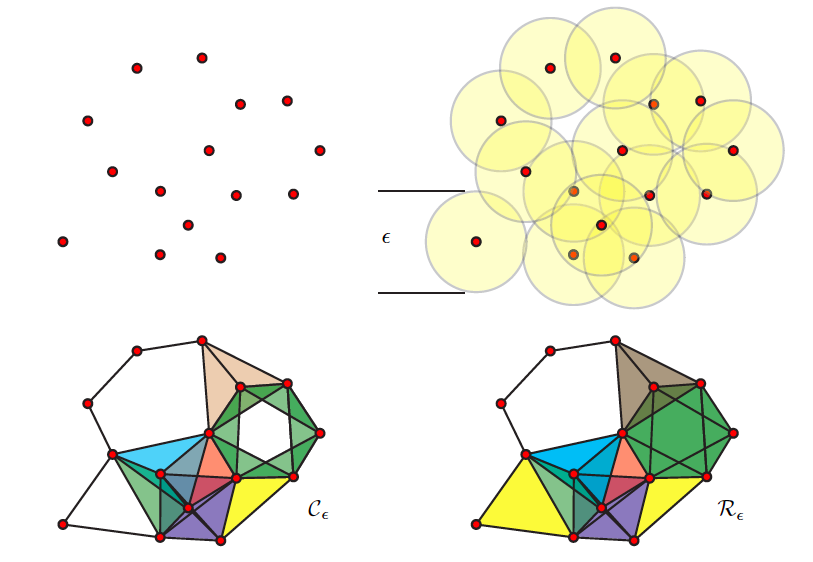
\includegraphics[width=0.75\textwidth]{complexes.png}\\
		\caption{Комплексы Чеха и Вьеториса—Рипса}
		\label{complexes}
	\end{center}
\end{figure}

Везде выше параметр $\tau$ был зафиксирован, но его можно изменять. Вслед за этим будут меняться и симплициальные комплексы, построенные с учетом $\tau$. {\it Фильтрацией симплициального комплекса $K$} называют вложенное семейство подкомплексов $ (K_\tau)_{\tau \in T} $, где $ T \subseteq \mathbb{R} $, такое, что если $ \tau < \tau^{'} $, то $ K_\tau \subseteq K_{\tau^{'}} $. Пример такой фильтрации изображен на рис. \ref{ripsfilt}, где изображения фильтрация симплициальных комплексов Рипса $\Rips_\tau(X)$.

\begin{figure}[!htbp]
	\begin{center}
		
\includegraphics[width=0.75\textwidth]{filtration.png}\\
		\caption{Фильтрация Рипса}
		\label{ripsfilt}
	\end{center}
\end{figure}

Имея фильтрацию $(K_\tau)_{\tau \in T}$, можно отслеживать изменение $H_k(K_\tau)$ с ростом $\tau$: могут появляться новые компоненты связности, уже существующие могут объединяться в одну компоненту, могут появляться циклы и "пустоты", соответствующие $1$ и $2$ группе гомологий. 
\begin{definition}
	$k$-ыми устойчивыми гомологиями фильтрованного комплекса $ (K_\tau)_{\tau \in T} $ называют  проиндексированное семейство абелевых групп $H_n(T) = \{ (H_n(K_\tau))_{\tau \in T} $ вместе с семейством гомоморфизмов $ (H_n(K_\tau) \to H_n(K_\tau^{'}))_{\tau \leq \tau^{'}} \}$.
\end{definition}
Такое семейство абелевых групп вместе с морфизмами на самом деле является примером  персистентного $\mathbb{Z}$-модуля($\mathbb{Z}$-модуля устойчивости): {\it персистентным $R$-модулем} $(A_*, x) $ называют последовательность $R$-модулей и гомоморфизмов между ними (над целочисленной временной шкалой $\mathbb{Z}_{\geq0}$).
\begin{center}
	\begin{tikzcd}[cells={nodes={minimum height=2em}}]
	A_0 \arrow[r, "x"] & A_1 \arrow[r,"x"]  &  A_2 \arrow[r,"x"] &  A_3 \arrow[r, "x"] & ... 
	\end{tikzcd}
\end{center}
Основная теорема про персистентные модули -- это структурная теорема. По аналогии с обычными модулями, она формулируется в терминах {\it конечнопорожденного} модуля устойчивости, т.е. такого модуля $(A_*, x)$, у которого существует конечный набор $a_1, ..., a_k \in A_*$ элементов, что любой элемент $a \in A_*$ можно выразить в виде линейной комбинации элементов вида $x^sa_r = x \circ ... \circ x(a_r)$.  Для ее формулировки понадобится еще пару определений: если $0 \leq j < s$, то {\it интервальным модулем устойчивости $I_{[j,s)}$} называют модуль устойчивости вида
\begin{center}
	\begin{tikzcd}[cells={nodes={minimum height=2em}}]
	0 \arrow[r] & ... \arrow[r]  &  0 \arrow[r] &  \underset{j}{R} \arrow[r, "id_R"] &  \underset{j+1}{R} \arrow[r, "id_R"] &
	... \arrow[r, "id_R"] & \underset{s-1}{R} \arrow[r, "0"] & \underset{s}{0} \arrow[r] & ... 
	\end{tikzcd}
\end{center}
Аналогично определяется бесконечный интервальный модуль $I_{[j, \infty)}$
\begin{center}
	\begin{tikzcd}[cells={nodes={minimum height=2em}}]
	0 \arrow[r] & ... \arrow[r]  &  0 \arrow[r] &  \underset{j}{R} \arrow[r, "id_R"] &  \underset{j+1}{R} \arrow[r, "id_R"] &
	... \arrow[r, "id_R"] & R \arrow[r, "id_R"] &  ... 
	\end{tikzcd}
\end{center}
Можно определить прямую сумму персистентных модулей: $ (A_*, x) \oplus (B_*, x) = ((A_* \oplus B_*), x) $, где $(A_* \oplus B_*)_j = A_j \oplus B_j$, а $x$ действует на каждом из слагаемых по отдельности.
\begin{theorem*}[об интервальном разложении] Пусть $R$ -- произвольное поле, а $(A_*, x)$ -- конечнопорожденный персистентный $R$-модуль. Тогда $(A_*, x)$ имеет единственное с точностью до перестановки слагаемых представление в виде прямой суммы конечного числа интервальный модулей:
	\[
		(A_*, x) \simeq \big( \bigoplus\limits_{k} I_{[j_k, s_k]} \big) 
																		\oplus 
						\big( \bigoplus\limits_{k} I_{[r_k, \infty)} \big)
	\]
\end{theorem*}

Так как персистентные гомологии -- это типичный пример конечнопорожденного персистентного модуля, то к нему можно применить структурную теорему. Из теоремы следует, что любой конечнопорожденный персистентный модуль с коэффициентами в поле, а значит и персистентные гомологии, можно закодировать в виде баркода (рис. \ref{barcode}) -- диаграммы, которая содержит интервалы, которые отвечают за время жизни свойств, которые как раз и характеризуются персистентными гомологиями.
\begin{figure}[]
	\begin{center}
		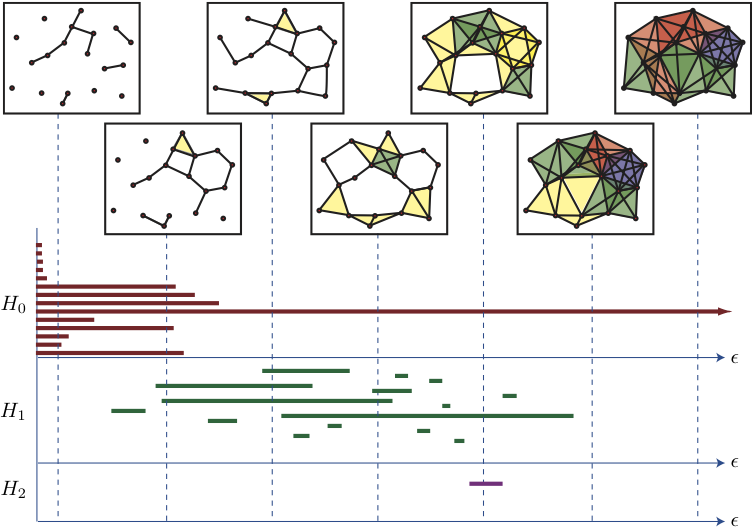
\includegraphics[width=0.75\textwidth]{barcode.png}\\
		\caption{Баркод}
		%\emph{Рис. 2. Баркод}
		\label{barcode}
	\end{center}
\end{figure}
\newline
Эту же информацию можно закодировать в виде диаграммы персистентности(диаграммы устойчивости) (рис. \ref{persist_diag}). Она строится следующим образом: каждый интервал баркода имеет начало $t_{birth}$ и конец $t_{death}$. На персистентной диаграмме каждый интервал баркода изображается в виде точки с координатами ($t_{birth}, t_{death}$), и каждая такая точка соответствует одному из слагаемых $I_{[j_k, s_k]}$ и $I_{[r_k, \infty)} $ из разложения. Таким образом, диаграмма устойчивости $B$ -- это множество $\{ (x,y) \in \mathbb{R} \times \mathbb{R} \cup \infty | x \leq y\}$. Чем дальше точка на персистентной диаграмме от диагонали, тем она важнее -- эта точка сигнализирует о наличии "$n$-мерной дырки". 
\begin{figure}[]
	\begin{center}
		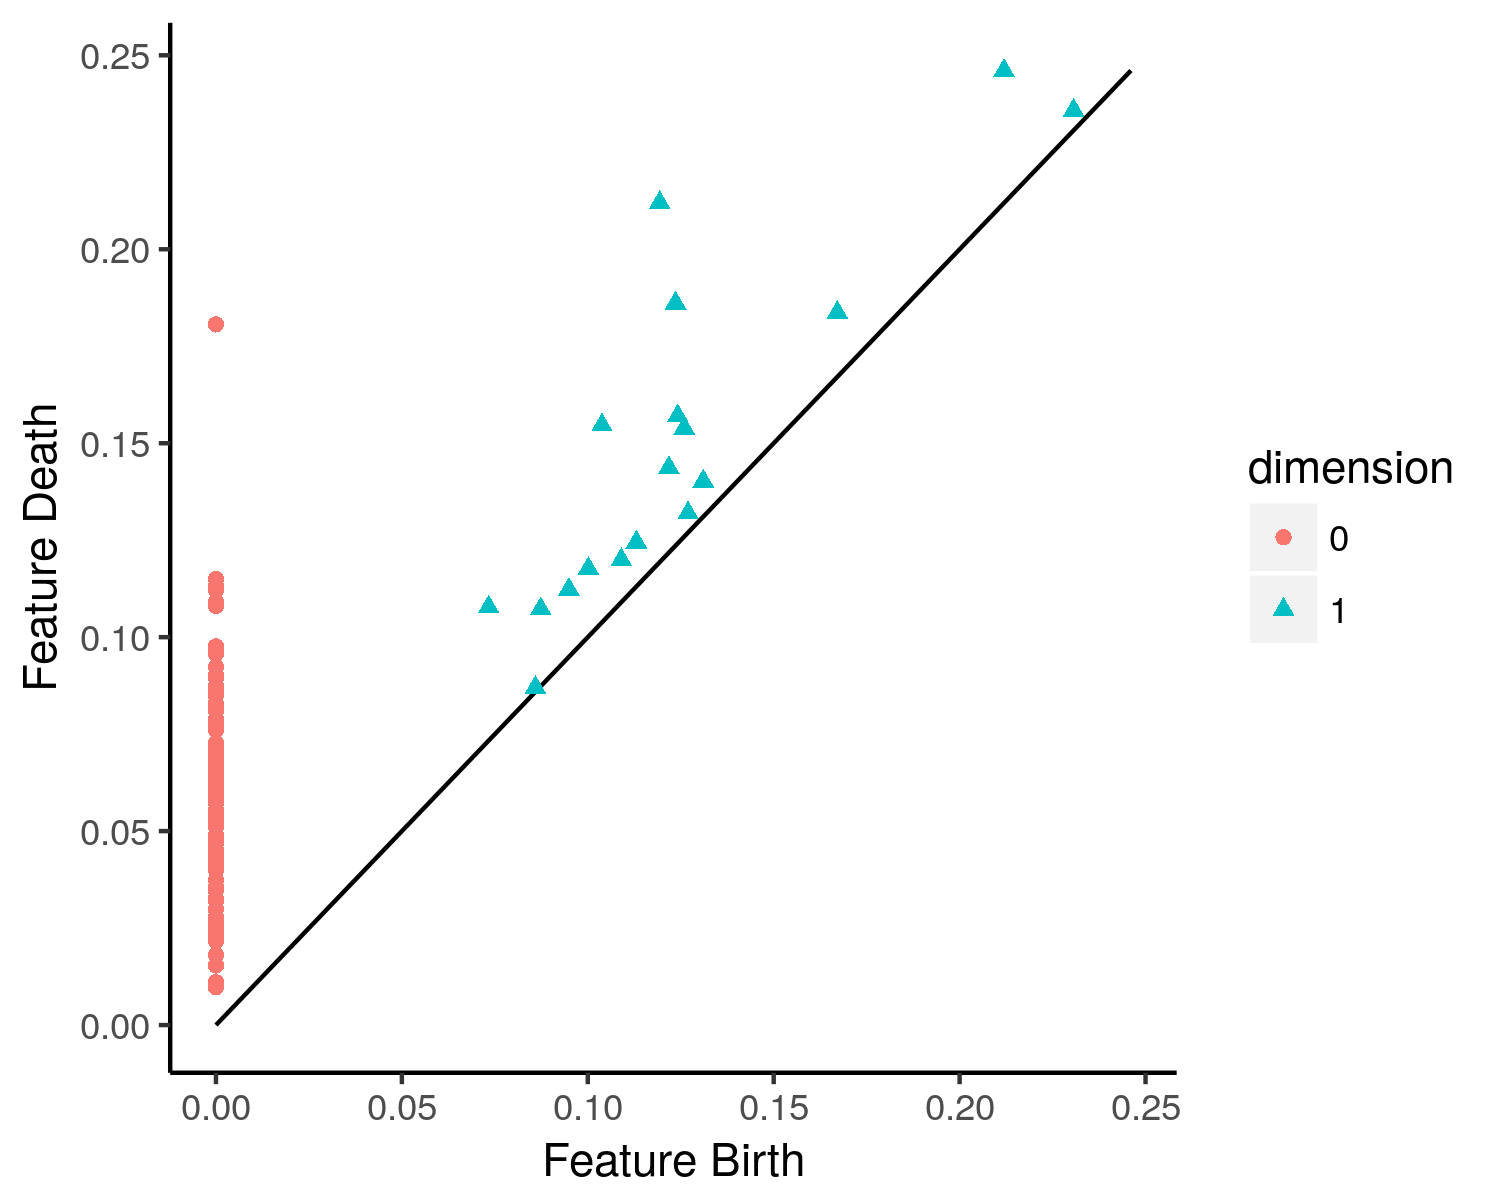
\includegraphics[width=0.75\textwidth]{persist_diag.png}\\
		\caption{Персистентная диаграмма}
		%\emph{Рис. 3. Персистентная диаграмма}
		\label{persist_diag}
	\end{center}
\end{figure}

\subsection{Векторные представления}
Как было показано выше, диаграмма устойчивости кодирует топологическую информацию. Кажется естественным, что такую топологическую информацию можно использовать во многих задачах анализа данных и машинного обучения. Однако для этого необходимо что-то знать про множество всех устойчивых диаграмм.

Пусть $\mathcal{D}$ -- множество устойчивых диаграмм. На нем можно ввести (естественную) метрику:
\[
W_p(B, B^{'}) = \inf\limits_{\gamma:B\to B^{'}} 
\big( 
\sum\limits_{u \in B} \norm{u - \gamma(u)}_\infty^p
\big) ^{\frac{1}{p}},
\]
где где $1 \leq p < \infty$, $B, B^{'}$ -- диаграммы персистентности. Такую метрику называют {\it $p-$метрику Васерштейна}. Другой естественной метрикой является т.н. {\it bottleneck distance} $W_\infty$:
\[
W_\infty(B, B^{'}) = \inf\limits_{\gamma:B\to B^{'}} \sup\limits_{u \in B}
\norm{u - \gamma(u)}_\infty.
\]
Таким образом, $\mathcal{D}$ с любой из указанных выше метрик образует метрическое пространство. 

Несложно увидеть, что, к сожалению, оно не является полным: пусть $x_n = (0, 2^{-n}) \in \mathbb{R}^2$ и $B_n = \{x_i\}_{i=1}^n$ -- диаграмма устойчивости. Тогда
\[
	W_p(B_n, B_{n+k}) \leq \frac{1}{2^{n+k}},
\]
а значит $\{B_n\}$ фундаментальна. Однако при $n \to \infty$ число недиагональных элементов в $B_n$ уходит в бесконечность, поэтому у последовательности диаграмм нет предела. 

Можно немного изменить определение устойчивых диаграмм -- пусть теперь у нас всегда она содержит диагональ $\Delta = \{(x,y) \in \mathbb{R}^2 | x=y\}$. Для таких диаграмм $p$-метрика Васерштейна обобщается естественным способом. Пустую диаграмму, содержащую только диагональ, будем обозначать через $B_\emptyset$. Тогда пространством устойчивых диаграмм можно считать следующее пространство:
\[
	\mathcal{D} \{ B | W_p(B, B_\emptyset) \textless \infty \}.
\]
Тогда, как показано в \cite{prop_measures}, такое пространство уже обладает хорошими свойствами, например оно полно и сепарабельно.

Однако для большинства алгоритмов машинного обучения и анализа данных этого недостаточно. Например, для метода опорных векторов необходимо, чтобы пространство признаков было гильбертовым(например, евклидовым), т.к. такой метод строит разделяющую гиперплоскость; деревья решений строят иерархическую модель "решений", которые, в свою очередь, также определяют гиперплоскость. 

Более того, в пространстве $\mathcal{D}$ устойчивых диаграмм, как также было показано в \cite{prop_measures}, даже такая стандартная статистика, как среднее арифметическое, для диаграмм устойчивости можно по-разному считать и интерпретировать. Например, если одна диаграмма, $B_1$, содержит 2 точки $B_1 = \{ (10, 22), (12, 20) \}$, а вторая диаграмма, $B_2$, содержит другие две точки $B_2 = \{ (10, 22), (12, 20) \}$, то что считать средним? Диаграмму $ \{ (11, 20), (11, 22) \}$ или $\{ (10,21), (12,21) \}$? Аналогичная ситуация обстоит и с дисперсией. 

Таким образом, геометрия пространства $\mathcal{D}$ персистентных диаграмм не позволяет комфортно с ними работать. Значит, для того, чтобы использовать диаграммы устойчивости в анализе данных и машинном обучении, нужно каким-то образом преобразовывать исходное пространство $\mathcal{D}$ диаграмм устойчивости в подходящее, например, гильбертово. Для этого существует несколько подходов. Далее опишем только те, что будут использоваться в данной работе -- это betti curves, persistent landscapes и heat kernel.

Итак, пусть $B = \{ (b_i, d_i) \}_{i=1}^n$ -- диаграмма персистентности. Тогда ее {\it Betti curve} назовем функцию $\beta_B: \mathbb{R} \to \mathbb{N} : t \mapsto \abs{\{(b_i, d_i) | b_i \le t \textless d_i\}}$. Иногда ее называют как persistence indicator function(PIF). Такие функции являются на самом деле ступенчатыми функциями, а потому образуют векторное пространство: суммой таких двух функций $\beta_B + \beta_C \coloneqq \beta_{B \cup C}$. На рис. \ref{betti-curve} показан график такой функции.

\begin{figure}[]
	\begin{center}
		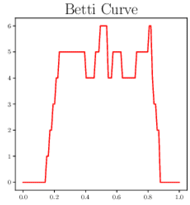
\includegraphics[width=0.3\textwidth]{betti-curve.png}\\
		\caption{График Betti curve}
		\label{betti-curve}
	\end{center}
\end{figure}

Как было показано выше, в пространстве персистентных диаграмм среднее не единственно. Но у Betti curve такой проблемы нет: для набора $\beta_1, ..., \beta_N$ Betti curves для устойчивых диаграмм $B_1, ..., B_N$ среднее $\bar\beta$ можно определить покомпонентно:
\[
	\bar\beta(t) = \frac{1}{N}\sum\limits_{i=1}^{N} \beta_i(t).
\]

В \cite{PIF} показано, что Betti curve устойчива относительно нормы $\norm{\beta}_1 = \int\limits_{\mathbb{R}} \abs{\beta(t)}dt$. Это означает, что небольшие изменения диаграммы приводят к небольшим изменениям Betti curve.

Пусть, все так же, $B = \{ (b_i, d_i) \}_{i=1}^n$ -- диаграмма персистентности. Тогда для каждой пары $(b_i, d_i)$ можно определить кусочно-линейную функцию $f_{(b_i, d_i)}: \mathbb{R} \to [0, \infty]$:
\[
	f_{(b_i, d_i)} : x \mapsto
	\left\{
		\begin{array}{ll}
			0, & \text{если } x \notin (b_i, d_i), \\
			x - b_i, & \text{если } x \in (b_i, \frac{b_i + d_i}{2}), \\
			-x + d, & \text{если } x \in (\frac{b+d}{2}, d)
		\end{array}
	\right.
\]
Тогда {\it persistent landscapes} диаграммы устойчивости $B$ -- это последовательность функций $\lambda_k : \mathbb{R} \to [0, \infty]$, где $k=1, 2, 3, ...$, и где $\lambda_k(x)$ -- это $k$-ое наибольшее значение последовательности $\{f_{(b_i, d_i)}(x)\}_{i=1}^n$, а если такого значения нет, то $\lambda_k=0$. Эквивалентно, можно определить persistent landscape как функцию $\lambda: \mathbb{N} \times \mathbb{R} \to [0, \infty]: (k,t) \mapsto \lambda_k(t)$. На рис. \ref{persist_land} представлен пример такого представления.

\begin{figure}[]
	\begin{center}
		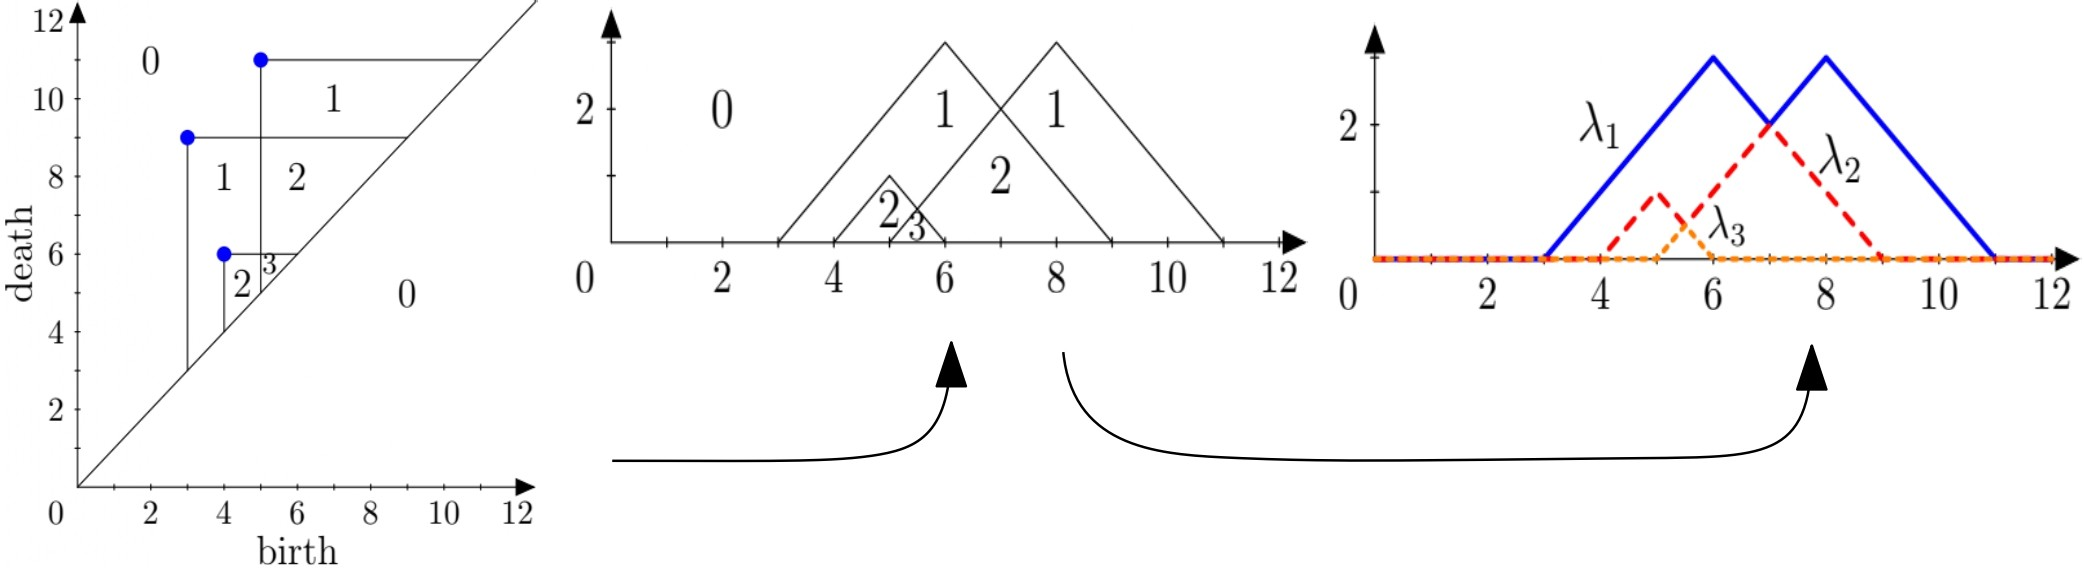
\includegraphics[width=0.75\textwidth]{persistent_landscape.jpeg}\\
		\caption{График persistent landscape}
		\label{persist_land}
	\end{center}
\end{figure}

Также как и Betti curves, для persistent landscapes можно посчитать среднее: пусть $\lambda^1, ..., \lambda^N$ -- persistent landscapes для $B_1, ..., B_N$ диаграмм. Тогда их среднее, $\bar\lambda$ можно определить покомпонентно:
\[
	\bar\lambda_k(t) \coloneqq \frac{1}{N}\sum\limits_{i=1}^{N} \lambda_k^i(t).
\]

Между persistent landscapes можно посчитать расстояние, например, используя $L^p$ норму:
\[
	\norm{\lambda - \lambda^{'}}_p = \big( \sum\limits_{k=1}^{\infty} \int \abs{ \lambda_k(t) - \lambda_k^{'}(t) }^p dt \big)^{\frac{1}{p}}.
\]

В \cite{pers_land} показано, что persistent landscape устойчива относительно метрики $L^p$ для $1 \le p \le \infty$. Это означает, что небольшие изменения диаграммы приводят к небольшим изменениям persistent landscape. 

Также рассматриваем $B = \{ (b_i, d_i) \}_{i=1}^n$ -- диаграмму персистентности. Определим для нее heat kernel. Напомним, что если $X$ -- некоторое множество, то функция $k: X \times X \to \mathbb{R}$ является {\it ядром(kernel)}, если существует Гильбертово пространство $\mathcal{H}$ и отображение(т.н. feature map) $\Phi:X \to \mathcal{H}$, такое, что $\forall x, y$ имеет место $k(x,y) = \langle \Phi(x), \Phi(y) \rangle_\mathcal{H}$, т.е. следующая диаграмма коммутативна:

\[
\begin{tikzcd}
&X \arrow[rr,"\Phi"] &[-1.5em] &[-1.5em] H \\
X \times X \arrow[dr,"\pi_X"'] \arrow[ur,"\pi_X"] \arrow[rr,"k"] &&
\mathbb{R} &&
\mathcal{H} \times \mathcal{H} \arrow[ul,"\pi_\mathcal{H}"']
\arrow[dl,"\pi_\mathcal{H}"] \arrow[ll,"{\langle \cdot, \cdot \rangle_\mathcal{H}}"'] \\
&X \arrow[rr,"\Phi"] && H
\end{tikzcd}
\]

Заметим, что диаграмма устойчивости $B$ можно единственным образом сопоставить сумму распределений дельта-функций Дирака в каждой точке диаграммы. Такой взгляд на диаграмму устойчивости позволяет каноническим образом получить структуру Гильбертова пространства. Тогда для данной диаграммы устойчивости $B$ можно рассмотреть следующее уравнение теплопроводности с граничным условием Дирихле:
\[
\begin{array}{ll}
	\Delta_x u = \partial_t u, & (x,t) \in \mathrm{Int}(\Omega \times \mathbb{R}_{\geq 0}), \\
	u = 0, & (x,t) \in \partial\Omega \times \mathbb{R}_{\geq 0}), \\
	u = \sum\limits_{x \in B} \delta_x, & (x,t) \in \Omega \times \{0\},
\end{array}
\]
где $\delta_x$ -- дельта-функция Дирака в точке $x$, а $\Omega = \{ (x_1, x_2) | x_1 \leq x_2 \} \subset \mathbb{R}^2$. Тогда решение данного уравнения -- функция в $L_2(\Omega)$, а значит можно рассмотреть отображение $F_\sigma: \mathcal{D} \to L_2(\Omega): B \mapsto \restr{u}{t=\sigma}$. Заметим, что $F_\sigma$ инъективно. Таким образом, можно определить ядро $k_\sigma: \mathcal{D} \times \mathcal{D} \to \mathbb{R}: (B, C) \mapsto \langle \Phi_\sigma(B), \Phi_\sigma(C) \rangle_{L_2(\Omega)}$. В \cite{heat_kernel} приведена мотивация построения именно такого ядра. также в \cite{heat_kernel} показано, что $k_\sigma$ устойчива относительно $1-$ метрики Васерштейна.

Все описанные выше методы сопоставляют диаграмме устойчивости некоторую функцию в Банаховом пространстве. Эти методы являются примерами векторизации. {\it Векторизацией} на множестве $X$ называют отображение $\varphi: X \to V$, где $V$ -- векторное пространство. Имея такую векторизацию, можно определить {\it амплитуду}: отображение $A: X \to \mathbb{R}: x \mapsto \norm{\varphi(x)}$, где $\varphi: X \to V$ -- векторизация множества $X$ на нормированное векторное пространство. Таким образом, для каждой диаграммы, выбрав определенную векторизацию, можно получить ее амплитуду, т.е. каждой диаграмме сопоставить некоторое вещественное число. Другой способ это сделать -- это посчитать т.н. {\it персистентную энтропию} -- это мера энтропии по Шеннону точек на диаграмме персистентности:
\[
E(B) = - \sum\limits_{i \in I} p_i \log(p_i), \text{ где $p_i = \dfrac{d_i - b_i}{\sum\limits_{i \in I}d_i-b_i}$. }
\]

Более подробно с персистентной энтропией можно ознакомиться в \cite{pers-entr}. Тогда, получив такие значения, из них можно сделать вектор в $\mathbb{R}^d$, который будет соответствовать диаграмме устойчивости. Такой вектор уже можно будет использовать в задачах анализа данных и машинного обучения.